%File: formatting-instructions-latex-2024.tex
%release 2024.0
\documentclass[letterpaper]{article} % DO NOT CHANGE THIS
\usepackage{aaai24}  % DO NOT CHANGE THIS
\usepackage{times}  % DO NOT CHANGE THIS
\usepackage{helvet}  % DO NOT CHANGE THIS
\usepackage{courier}  % DO NOT CHANGE THIS
\usepackage[hyphens]{url}  % DO NOT CHANGE THIS
\usepackage{graphicx} % DO NOT CHANGE THIS
\usepackage{indentfirst}
\usepackage[portuguese]{babel}
\urlstyle{rm} % DO NOT CHANGE THIS
\def\UrlFont{\rm}  % DO NOT CHANGE THIS
\usepackage{natbib}  % DO NOT CHANGE THIS AND DO NOT ADD ANY OPTIONS TO IT
\usepackage{caption} % DO NOT CHANGE THIS AND DO NOT ADD ANY OPTIONS TO IT
\frenchspacing  % DO NOT CHANGE THIS
\setlength{\pdfpagewidth}{8.5in}  % DO NOT CHANGE THIS
\setlength{\pdfpageheight}{11in}  % DO NOT CHANGE THIS
%
% These are recommended to typeset algorithms but not required. See the subsubsection on algorithms. Remove them if you don't have algorithms in your paper.
\usepackage{algorithm}
\usepackage{algorithmic}

%
% These are are recommended to typeset listings but not required. See the subsubsection on listing. Remove this block if you don't have listings in your paper.
\usepackage{newfloat}
\usepackage{listings}
\DeclareCaptionStyle{ruled}{labelfont=normalfont,labelsep=colon,strut=off} % DO NOT CHANGE THIS
\lstset{%
	basicstyle={\footnotesize\ttfamily},% footnotesize acceptable for monospace
	numbers=left,numberstyle=\footnotesize,xleftmargin=2em,% show line numbers, remove this entire line if you don't want the numbers.
	aboveskip=0pt,belowskip=0pt,%
	showstringspaces=false,tabsize=2,breaklines=true}
\floatstyle{ruled}
\newfloat{listing}{tb}{lst}{}
\floatname{listing}{Listing}
%
% Keep the \pdfinfo as shown here. There's no need
% for you to add the /Title and /Author tags.
\pdfinfo{
/TemplateVersion (2024.1)
}

% DISALLOWED PACKAGES
% \usepackage{authblk} -- This package is specifically forbidden
% \usepackage{balance} -- This package is specifically forbidden
% \usepackage{color (if used in text)
% \usepackage{CJK} -- This package is specifically forbidden
% \usepackage{float} -- This package is specifically forbidden
% \usepackage{flushend} -- This package is specifically forbidden
% \usepackage{fontenc} -- This package is specifically forbidden
% \usepackage{fullpage} -- This package is specifically forbidden
% \usepackage{geometry} -- This package is specifically forbidden
% \usepackage{grffile} -- This package is specifically forbidden
% \usepackage{hyperref} -- This package is specifically forbidden
% \usepackage{navigator} -- This package is specifically forbidden
% (or any other package that embeds links such as navigator or hyperref)
% \indentfirst} -- This package is specifically forbidden
% \layout} -- This package is specifically forbidden
% \multicol} -- This package is specifically forbidden
% \nameref} -- This package is specifically forbidden
% \usepackage{savetrees} -- This package is specifically forbidden
% \usepackage{setspace} -- This package is specifically forbidden
% \usepackage{stfloats} -- This package is specifically forbidden
% \usepackage{tabu} -- This package is specifically forbidden
% \usepackage{titlesec} -- This package is specifically forbidden
% \usepackage{tocbibind} -- This package is specifically forbidden
% \usepackage{ulem} -- This package is specifically forbidden
% \usepackage{wrapfig} -- This package is specifically forbidden
% DISALLOWED COMMANDS
% \nocopyright -- Your paper will not be published if you use this command
% \addtolength -- This command may not be used
% \balance -- This command may not be used
% \baselinestretch -- Your paper will not be published if you use this command
% \clearpage -- No page breaks of any kind may be used for the final version of your paper
% \columnsep -- This command may not be used
% \newpage -- No page breaks of any kind may be used for the final version of your paper
% \pagebreak -- No page breaks of any kind may be used for the final version of your paperr
% \pagestyle -- This command may not be used
% \tiny -- This is not an acceptable font size.
% \vspace{- -- No negative value may be used in proximity of a caption, figure, table, section, subsection, subsubsection, or reference
% \vskip{- -- No negative value may be used to alter spacing above or below a caption, figure, table, section, subsection, subsubsection, or reference

\setcounter{secnumdepth}{2} %May be changed to 1 or 2 if section numbers are desired.

% The file aaai24.sty is the style file for AAAI Press
% proceedings, working notes, and technical reports.
%

% Title


\title{Universidade Federal de Minas Gerais \\[10pt]
DCC642 - Introdução à Inteligência Artificial (2025/2) \\
 TP1: Busca no Espaço de Estados}
\author {
    Raphael Henrique Braga Leivas - 2020028101
}


\begin{document}

\maketitle


\section{Introdução}

O presente trabalho busca documentar

\section{Objetivos}

\section{Casos de Teste}

Nessa seção são abordados 7 casos de teste para evidenciar as principais 
diferenças entre os algoritmos estudados.


\subsection{BFS não é ótimo}

O BFS não garante otimalidade se os custos forem diferentes, como 
mostra a Figura \ref{fig:BFS_nao_otimo}.

\begin{figure}[htb]
	\centering 
    \caption{Caso em que o BFS não é ótimo. (a) Mapa inicial, (b)
	caminho retornado pelo BFS, (c) caminho ótimo encontrado pelo UCS.}
	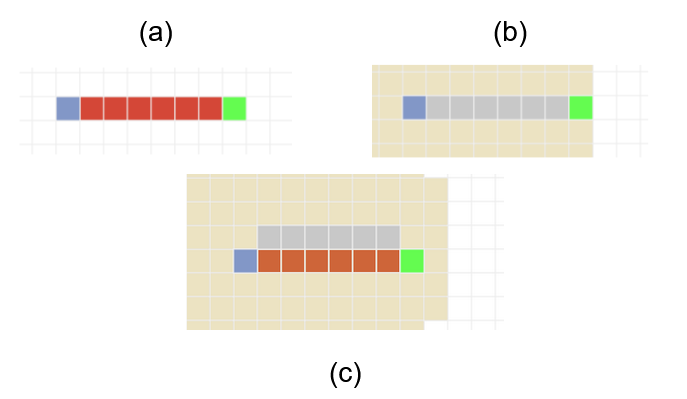
\includegraphics[width=\columnwidth]{images/BFS_nao_otimo.png}
	\label{fig:BFS_nao_otimo}
\end{figure}

Na Figura \ref{fig:BFS_nao_otimo} (a), temos que o caminho direto do início ao alvo 
passa por casas de custo elevado (9), enquanto as demais casas possuem custo unitário.
O BFS, por explorar os nós em camadas, acaba encontrando o caminho (b) que vai diretamente 
até o alvo, passando pelos nós custosos e retornando um caminho de custo total 55.

Contudo, claramente existe um camingo melhor que passa pelos nós de custo unitário.
Assim, usando o UCS é possível encontrar o caminho da Figura \ref{fig:BFS_nao_otimo} (c), 
com custo total 8, que é a solução ótima para o problema.

\subsection{BFS é equivalente à UCS}

BFS e UCS são equivalentes quando todos os custos são iguais, como mostra 
a Figura \ref{fig:BFS_UCS_equiv} (a). Todas as arestas do mapa possuem
 custo unitário, de modo que a solução encontrada pelo BFS na Figura \ref{fig:BFS_UCS_equiv} (b) 
 é igual à solução do UCS na Figura \ref{fig:BFS_UCS_equiv} (c). Além disso, note que 
 a maneira em que os nós são explorados é bastante parecida, avançando radialmente 
 a partir do nó inicial.


\begin{figure}[htb]
	\centering 
    \caption{Caso em que o BFS e o UCS são equivalentes. (a) Mapa inicial, (b)
	caminho retornado pelo BFS, (c) caminho retornado pelo UCS.}
	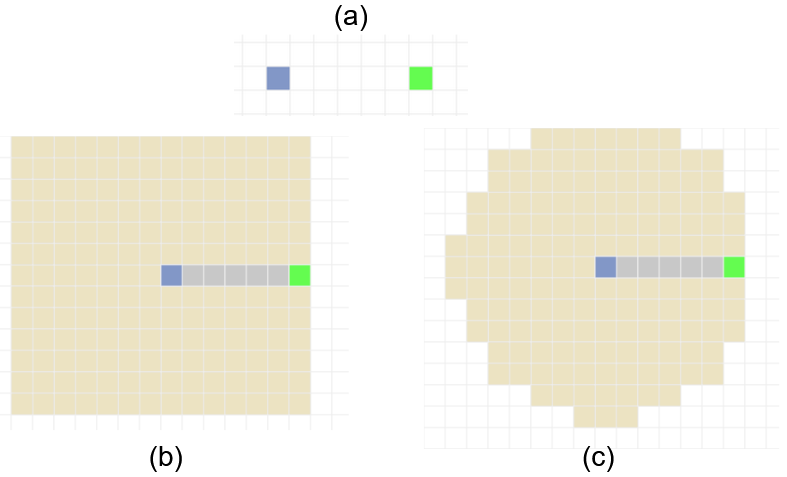
\includegraphics[width=\columnwidth]{images/BFS_UCS_equiv.png}
	\label{fig:BFS_UCS_equiv}
\end{figure}


\subsection{DFS retorna a solução ótima}

O DFS em geral não é ótimo uma vez que ele retorna o primeiro caminho encontrado
e não necessariamente o de menor custo. Contudo, em alguns casos o DFS pode
retornar a solução ótima, como mostra a Figura \ref{fig:DFS_otimo} (a), em que 
todos os custos são iguais e todas as soluções possíveis possuem a mesma 
profundidade.

\begin{figure}[htb]
	\centering 
    \caption{Caso em que o DFS garante otimalidade. (a) Mapa inicial, (b)
	caminho retornado pelo DFS.}
	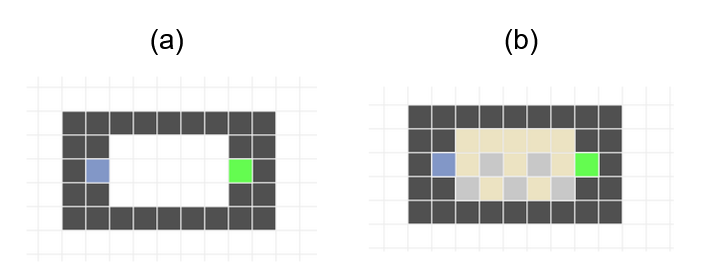
\includegraphics[width=\columnwidth]{images/DFS_otimo.png}
	\label{fig:DFS_otimo}
\end{figure}

Note que esse caso é bastante específico e não é possível garantir que o DFS
sempre retorne a solução ótima. 

\subsection{Greedy é ótimo}

A busca gulosa pela melhor escolha (Greedy) é ótima se 

\subsection{Greedy não é ótimo}


\subsection{A* é melhor que UCS}

\subsection{A* é equivalente à UCS}

\section{Conclusão}


\bibliography{aaai24}

\end{document}
